\documentclass{article}
\usepackage{graphicx} % Required for inserting images
\usepackage[utf8]{inputenc}
\usepackage[T1]{fontenc}
\usepackage{karnaugh-map}
\usepackage[polish]{babel}
\usepackage{subcaption}
\usepackage{float}
\usepackage{enumitem}
\usepackage{url}


\begin{document}

\begin{center}
    % Zamiast 'p{0.7\textwidth}|l|' używamy dwóch kolumn 'p{...}'
    % To daje nam pełną kontrolę nad szerokością i zawijaniem tekstu.
    % Suma (np. 0.65 + 0.3 = 0.95) musi być mniejsza niż 1.0
    
    \begin{tabular}{|p{0.65\textwidth}|p{0.3\textwidth}|}
        \hline
        
        % --- PIERWSZY WIERSZ LOGICZNY (wg obrazka) ---
        
        % Komórka 1,1 (Lewa-góra)
        Wydział Informatyki Politechniki Białostockiej \newline
        Przedmiot: Modułowe systemy cyfrowe
        & 
        % Komórka 1,2 (Prawa-góra)
        Data: 28.10.2025 \\
        
        \hline % Linia oddzielająca wg obrazka
        
        % --- DRUGI WIERSZ LOGICZNY (wg obrazka) ---
        
        % Komórka 2,1 (Lewa-dół)
        Zajęcia nr 2 \newline
        Temat: Bloki kombinacyjne: multipleksery, demultipleksery i dekodery \newline
        \vspace{1em} % Dodatkowy odstęp dla czytelności
        Grupa: Lab 8 \newline
        Imię i nazwisko: \newline
        Kamil Kubajewski, Jakub Matusiewicz, Bartosz Orłowski
        & 
        % Komórka 2,2 (Prawa-dół)
        Prowadzący: \newline
        dr hab. inż. Sławomir Zieliński \\
        
        \hline
    \end{tabular}
\end{center}

\section{Cel ćwiczeń}

Zapoznanie z podstawowymi kombinacyjnymi układami scalonymi, konkretnie \textbf{multiplekserami}, \textbf{demultiplekserami} i \textbf{dekoderami}.

\section{Podstawa teoretyczna}

    \pagebreak

\pagebreak
\section{Przebieg ćwiczeń}
\subsection{Zadanie 1}
Zrealizować multiplekser dwuwejściowy na bramkach logicznych (DB10).
\begin{figure}[h]
    \centering
    \includegraphics[width=0.50\textwidth]{Obwod1_1.PNG}
    \caption{Obwód do zadania 1 i 2}
    \label{fig:moj_obrazek}
\end{figure}\\

Multiplekser dwuwejściowy posiada dwa wejścia danych oraz jedną linię sterującą. Jego budowa opiera się na dwóch bramkach \textbf{AND}, których wyjścia podłączone są do wejść dwuwejściowej bramki \textbf{OR}, co pozwala na wybór aktywnego wejścia. Do przetestowania układu użyto modułu \textbf{DB10}, wykorzystując przełączniki do zadawania stanów logicznych \textbf{0} lub \textbf{1} na wejściach i linii sterującej.

\subsection{Zadanie 2}
Zrealizować multiplekser czterowejściowy na bramkach logicznych (DB10).
\begin{figure}[h]
    \centering
    \includegraphics[width=0.50\textwidth]{Obwod1.PNG}
    \caption{Obwód do zadania 1 i 2}
    \label{fig:moj_obrazek}
\end{figure}\\
Multiplekser czterowejściowy posiada cztery wejścia danych oraz dwie linie sterujące. Jego budowa opiera się na czterech bramkach \textbf{AND}, których wyjścia podłączone są do wejść czterowejściowej bramki \textbf{OR}, co pozwala na wybór aktywnego wejścia. Do przetestowania układu użyto modułu \textbf{DB10}, wykorzystując przełączniki do zadawania stanów logicznych \textbf{0} lub \textbf{1} na wejściach i liniach sterujących.

\pagebreak
\subsection{Zadanie 3}
Zrealizować demultiplekser na bramkach logicznych (DB10)
\begin{figure}[h]
    \centering
    \includegraphics[width=0.50\textwidth]{Obwod2.PNG}
    \caption{Obwód do zadania 3}
    \label{fig:moj_obrazek}
\end{figure}\\
Demultiplekser jednowejściowy z czterema wyjściami składa się z jednego wejścia danych i dwóch linii sterujących. Podłączając bramkę NOT do wejść linii sterujących i cztery bramki AND, możemy kierować sygnał z wejścia na wybrane wyjście. Do przetestowania użyto modułu \textbf{DB10}, do którego podłączono przełączniki dla zmiany sygnałów 0 lub 1.

\subsection{Zadanie 4}
Przebadać blok funkcjonalny z dekoderem DB31. Zrealizować dekodery kodu 1 z 8 oraz 1 z
16.
\begin{figure}[h]
    \centering
    \includegraphics[width=0.50\textwidth]{Obwod2.PNG}
    \caption{Obwód do zadania 3}
    \label{fig:moj_obrazek}
\end{figure}

\pagebreak
\subsection{Zadanie 5}
Zrealizować dekoder kodu BCD z wyjściem na wyświetlacz 7 – segmentowy (DB15).
\begin{figure}[h]
    \centering
    \includegraphics[width=0.50\textwidth]{Obwod3.PNG}
    \caption{Obwód do zadania 5}
    \label{fig:moj_obrazek}
\end{figure}\\
Do przetestowania dekodera BCD na 7-segmentowy wyświetlacz użyto modułu \textbf{DB15}. Moduł ten zawiera układ scalony \textbf{74LS47} oraz zintegrowany \textbf{wyświetlacz 7-segmentowy}. Za pomocą przełączników podawano na wejścia $A_0$-$A_3$ układu 4-bitowe kombinacje kodu BCD, odpowiadające cyfrom od 0 do 9. Sprawdzono, że dla każdej podanej kombinacji na wyświetlaczu pojawiała się poprawna cyfra.

\pagebreak
\section{Dyskusja błedów}
%Klasyczna formułka np. z EDI, jaka powinna byc oczekiwana wartość? Bład ludzki, niedokładnosc przyrządów, itd

\pagebreak
\section{Wnioski}
\section{Literatura}

\renewcommand{\refname}{}

\begin{thebibliography}{9}
	
	\bibitem{maciak} 
	T. Maciak, \textit{Skrypt do laboratorium Elektroniki cyfrowej}, 
	Wydział Informatyki Politechniki Białostockiej, Białystok, 2021.
	
	\bibitem{wiki} 
	\textit{Transistor–transistor logic}, Wikipedia, dostęp online: 
	\url{https://en.wikipedia.org/wiki/Transistor-transistor_logic}, 
	data dostępu: październik 2025.
	
	\bibitem{wiki-flip} 
	\textit{Excitation table}, Wikipedia, dostęp online: 
	\url{https://en.wikipedia.org/wiki/Excitation_table}, 
	data dostępu: lipiec 2025.
	
	\bibitem{TI7400} 
	Texas Instruments, \textit{SN7400 NAND Gate Datasheet}, dostęp online: 
	\url{https://www.ti.com/lit/ds/symlink/sn7400.pdf}, 
	data dostępu: październik 2025.
	
\end{thebibliography}

\pagebreak
\section{Protokół}

\begin{figure}[h]
    \centering
    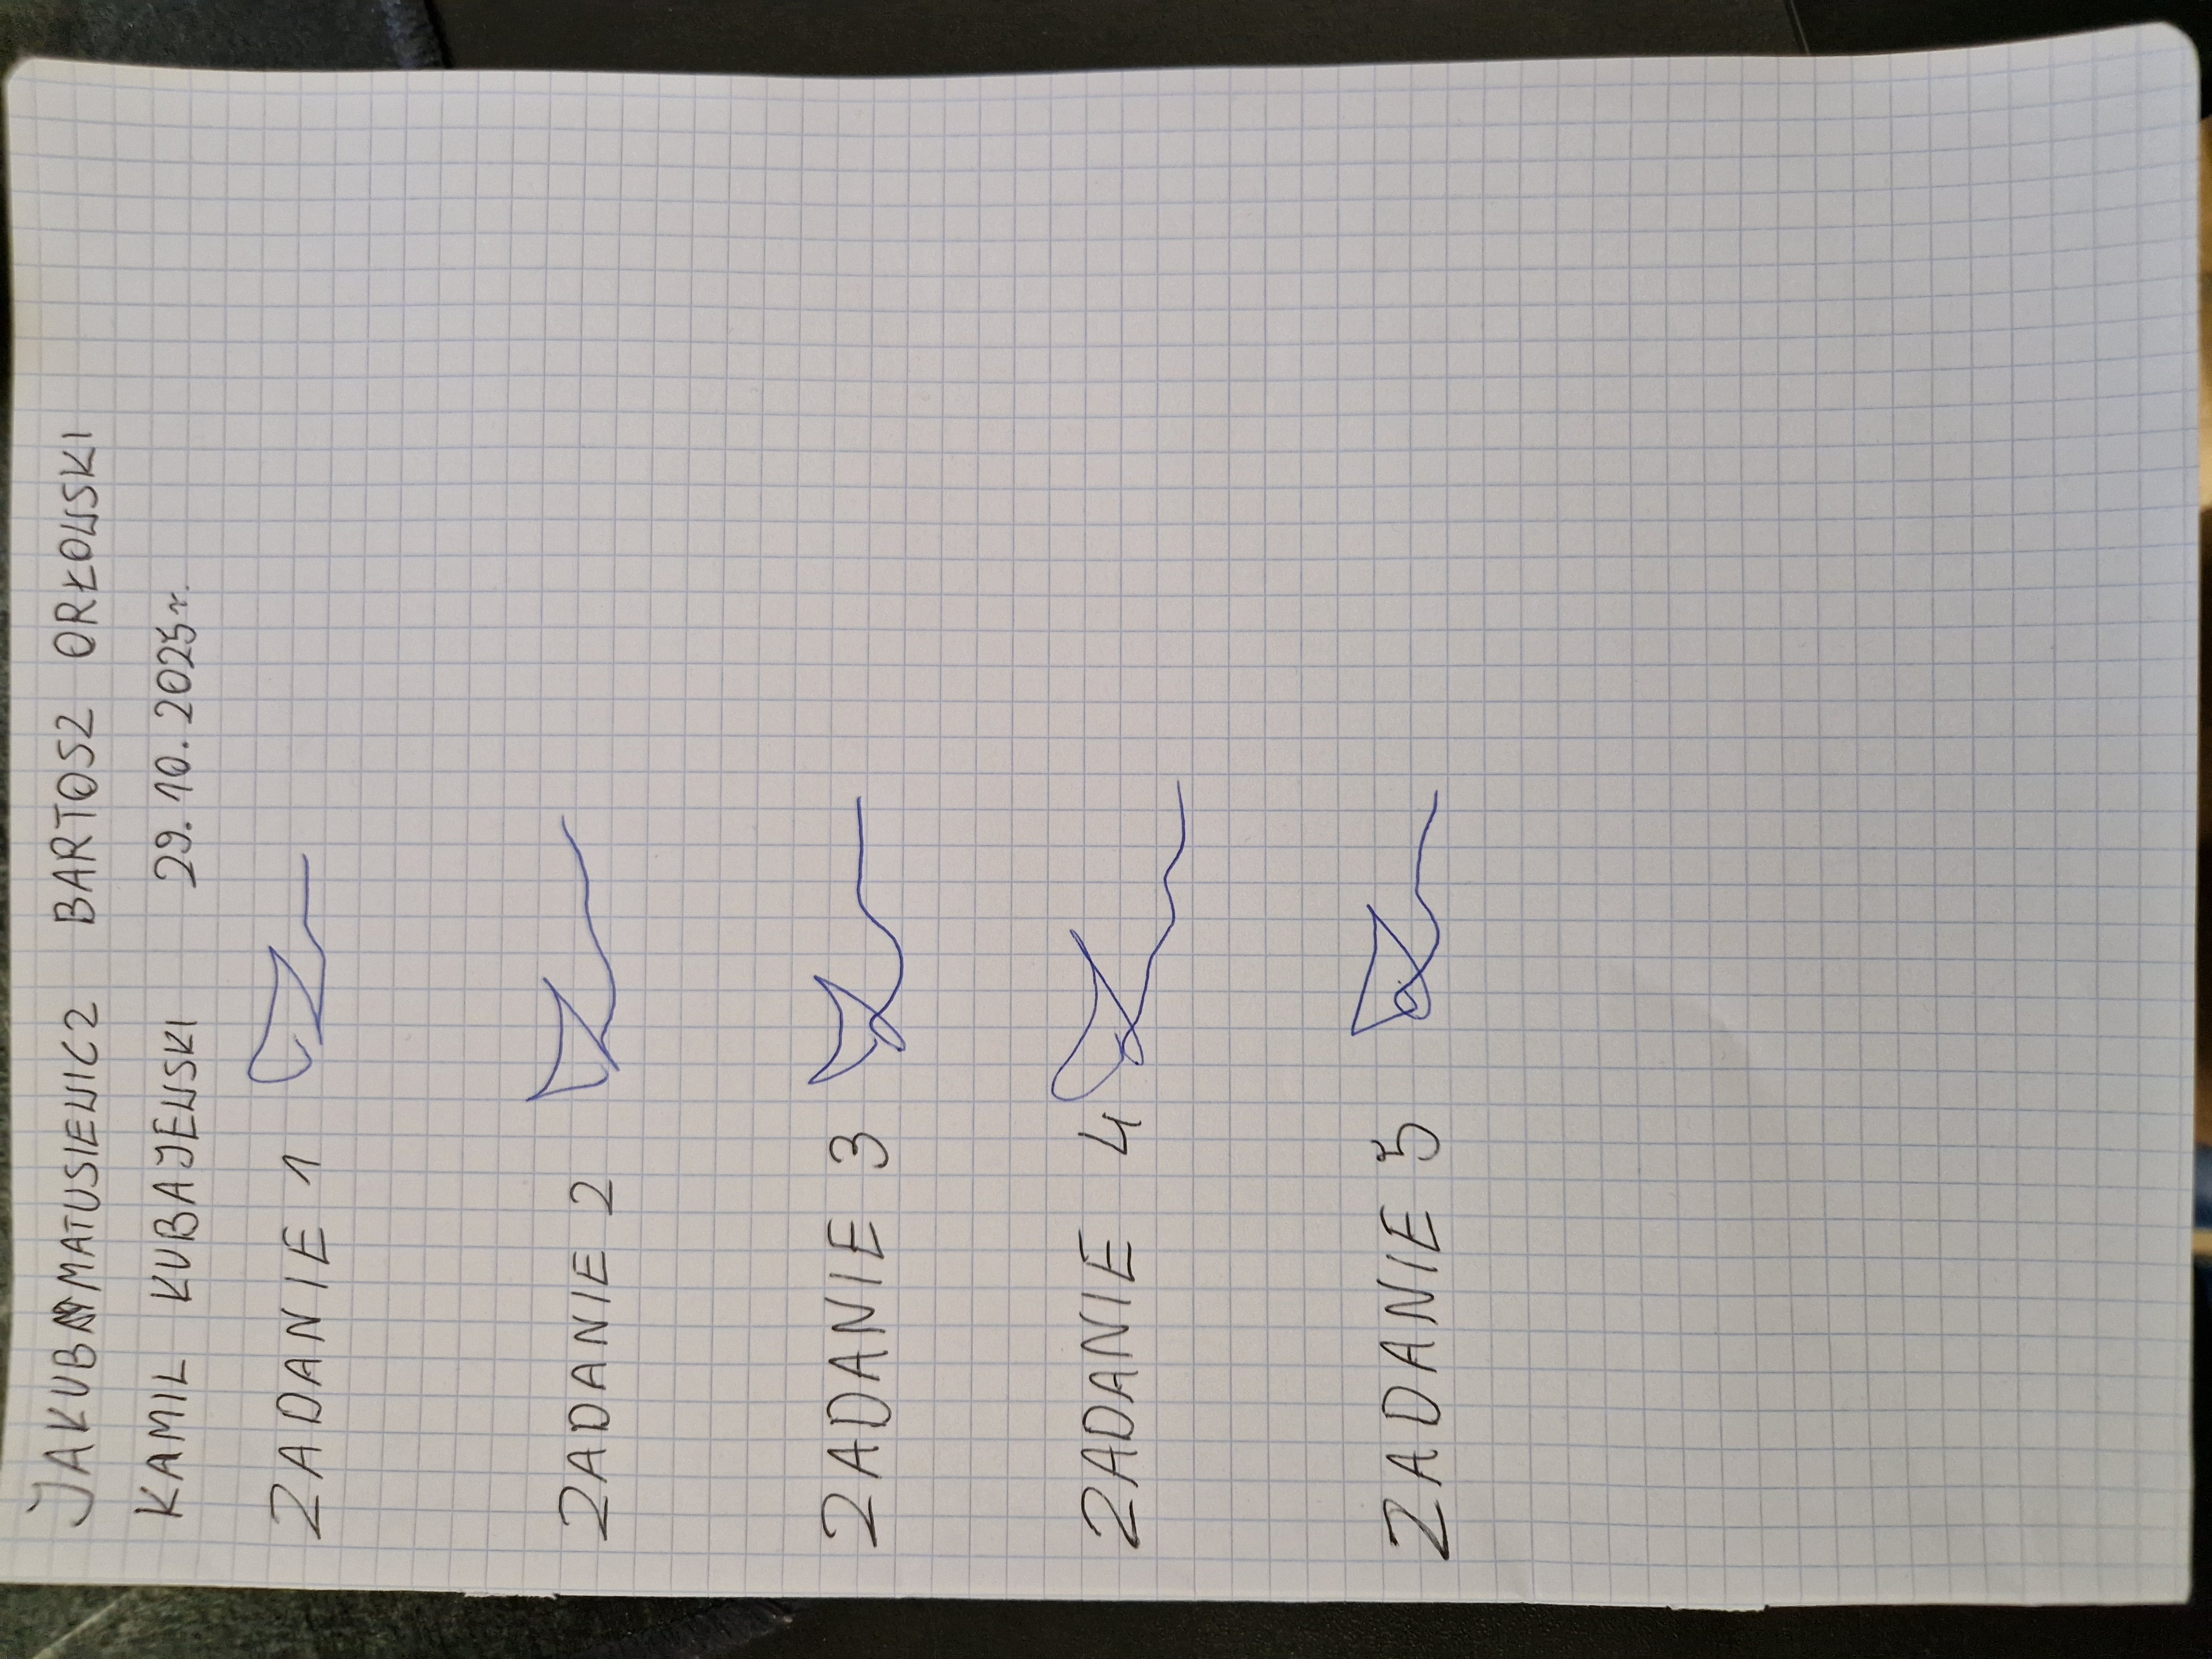
\includegraphics[width=1\textwidth, angle=-90]{protokol.JPG}
    \caption{Protokół}
    \label{fig:moj_obrazek}
\end{figure}
\end{document}